\documentclass[11pt,compress,t,notes=noshow, xcolor=table]{beamer}

\documentclass[11pt,compress,t,notes=noshow, xcolor=table]{beamer}
\usepackage[]{graphicx}\usepackage[]{color}
% maxwidth is the original width if it is less than linewidth
% otherwise use linewidth (to make sure the graphics do not exceed the margin)
\makeatletter
\def\maxwidth{ %
  \ifdim\Gin@nat@width>\linewidth
    \linewidth
  \else
    \Gin@nat@width
  \fi
}
\makeatother

\definecolor{fgcolor}{rgb}{0.345, 0.345, 0.345}
\newcommand{\hlnum}[1]{\textcolor[rgb]{0.686,0.059,0.569}{#1}}%
\newcommand{\hlstr}[1]{\textcolor[rgb]{0.192,0.494,0.8}{#1}}%
\newcommand{\hlcom}[1]{\textcolor[rgb]{0.678,0.584,0.686}{\textit{#1}}}%
\newcommand{\hlopt}[1]{\textcolor[rgb]{0,0,0}{#1}}%
\newcommand{\hlstd}[1]{\textcolor[rgb]{0.345,0.345,0.345}{#1}}%
\newcommand{\hlkwa}[1]{\textcolor[rgb]{0.161,0.373,0.58}{\textbf{#1}}}%
\newcommand{\hlkwb}[1]{\textcolor[rgb]{0.69,0.353,0.396}{#1}}%
\newcommand{\hlkwc}[1]{\textcolor[rgb]{0.333,0.667,0.333}{#1}}%
\newcommand{\hlkwd}[1]{\textcolor[rgb]{0.737,0.353,0.396}{\textbf{#1}}}%
\let\hlipl\hlkwb

\usepackage{framed}
\makeatletter
\newenvironment{kframe}{%
 \def\at@end@of@kframe{}%
 \ifinner\ifhmode%
  \def\at@end@of@kframe{\end{minipage}}%
  \begin{minipage}{\columnwidth}%
 \fi\fi%
 \def\FrameCommand##1{\hskip\@totalleftmargin \hskip-\fboxsep
 \colorbox{shadecolor}{##1}\hskip-\fboxsep
     % There is no \\@totalrightmargin, so:
     \hskip-\linewidth \hskip-\@totalleftmargin \hskip\columnwidth}%
 \MakeFramed {\advance\hsize-\width
   \@totalleftmargin\z@ \linewidth\hsize
   \@setminipage}}%
 {\par\unskip\endMakeFramed%
 \at@end@of@kframe}
\makeatother

\definecolor{shadecolor}{rgb}{.97, .97, .97}
\definecolor{messagecolor}{rgb}{0, 0, 0}
\definecolor{warningcolor}{rgb}{1, 0, 1}
\definecolor{errorcolor}{rgb}{1, 0, 0}
\newenvironment{knitrout}{}{} % an empty environment to be redefined in TeX

\usepackage{alltt}
\newcommand{\SweaveOpts}[1]{}  % do not interfere with LaTeX
\newcommand{\SweaveInput}[1]{} % because they are not real TeX commands
\newcommand{\Sexpr}[1]{}       % will only be parsed by R
\newcommand{\xmark}{\ding{55}}%


\usepackage[english]{babel}
\usepackage[utf8]{inputenc}

\usepackage{dsfont}
\usepackage{verbatim}
\usepackage{amsmath}
\usepackage{amsfonts}
\usepackage{amssymb}
\usepackage{bm}
\usepackage{csquotes}
\usepackage{multirow}
\usepackage{longtable}
\usepackage{booktabs}
\usepackage{enumerate}
\usepackage[absolute,overlay]{textpos}
\usepackage{psfrag}
\usepackage{algorithm}
\usepackage{algpseudocode}
\usepackage{eqnarray}
\usepackage{arydshln}
\usepackage{tabularx}
\usepackage{placeins}
\usepackage{tikz}
\usepackage{setspace}
\usepackage{colortbl}
\usepackage{mathtools}
\usepackage{wrapfig}
\usepackage{bm}
\usepackage{amsmath}
\usepackage{pifont}

\usetikzlibrary{shapes,arrows,automata,positioning,calc,chains,trees, shadows}
\tikzset{
  %Define standard arrow tip
  >=stealth',
  %Define style for boxes
  punkt/.style={
    rectangle,
    rounded corners,
    draw=black, very thick,
    text width=6.5em,
    minimum height=2em,
    text centered},
  % Define arrow style
  pil/.style={
    ->,
    thick,
    shorten <=2pt,
    shorten >=2pt,}
}

\usepackage{subfig}

% Defines macros and environments
\usepackage{../../style/lmu-lecture}


\let\code=\texttt
\let\proglang=\textsf

\setkeys{Gin}{width=0.9\textwidth}

\setbeamertemplate{frametitle}{\expandafter\uppercase\expandafter\insertframetitle}

\usepackage{bbm}
% basic latex stuff
\newcommand{\pkg}[1]{{\fontseries{b}\selectfont #1}} %fontstyle for R packages
\newcommand{\lz}{\vspace{0.5cm}} %vertical space
\newcommand{\dlz}{\vspace{1cm}} %double vertical space
\newcommand{\oneliner}[1] % Oneliner for important statements
{\begin{block}{}\begin{center}\begin{Large}#1\end{Large}\end{center}\end{block}}


%new environments
\newenvironment{vbframe}  %frame with breaks and verbatim
{
 \begin{frame}[containsverbatim,allowframebreaks]
}
{
\end{frame}
}

\newenvironment{vframe}  %frame with verbatim without breaks (to avoid numbering one slided frames)
{
 \begin{frame}[containsverbatim]
}
{
\end{frame}
}

\newenvironment{blocki}[1]   % itemize block
{
 \begin{block}{#1}\begin{itemize}
}
{
\end{itemize}\end{block}
}

\newenvironment{fragileframe}[2]{  %fragile frame with framebreaks
\begin{frame}[allowframebreaks, fragile, environment = fragileframe]
\frametitle{#1}
#2}
{\end{frame}}


\newcommand{\myframe}[2]{  %short for frame with framebreaks
\begin{frame}[allowframebreaks]
\frametitle{#1}
#2
\end{frame}}

\newcommand{\remark}[1]{
  \textbf{Remark:} #1
}


\newenvironment{deleteframe}
{
\begingroup
\usebackgroundtemplate{
\includegraphics[width=\paperwidth,height=\paperheight]{../style/color/red.png}}
 \begin{frame}
}
{
\end{frame}
\endgroup
}
\newenvironment{simplifyframe}
{
\begingroup
\usebackgroundtemplate{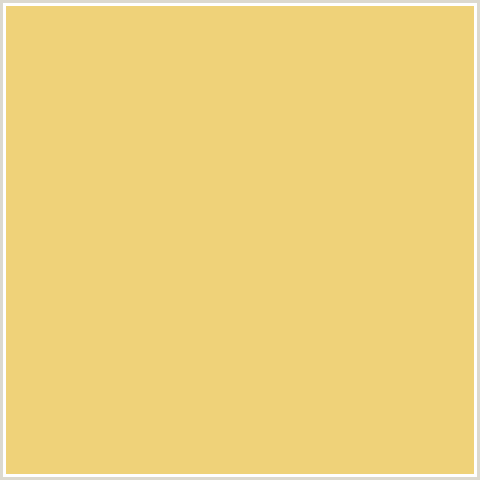
\includegraphics[width=\paperwidth,height=\paperheight]{../style/color/yellow.png}}
 \begin{frame}
}
{
\end{frame}
\endgroup
}\newenvironment{draftframe}
{
\begingroup
\usebackgroundtemplate{
\includegraphics[width=\paperwidth,height=\paperheight]{../style/color/green.jpg}}
 \begin{frame}
}
{
\end{frame}
\endgroup
}
% https://tex.stackexchange.com/a/261480: textcolor that works in mathmode
\makeatletter
\renewcommand*{\@textcolor}[3]{%
  \protect\leavevmode
  \begingroup
    \color#1{#2}#3%
  \endgroup
}
\makeatother





% math spaces
\ifdefined\N                                                                
\renewcommand{\N}{\mathds{N}} % N, naturals
\else \newcommand{\N}{\mathds{N}} \fi 
\newcommand{\Z}{\mathds{Z}} % Z, integers
\newcommand{\Q}{\mathds{Q}} % Q, rationals
\newcommand{\R}{\mathds{R}} % R, reals
\ifdefined\C 
  \renewcommand{\C}{\mathds{C}} % C, complex
\else \newcommand{\C}{\mathds{C}} \fi
\newcommand{\continuous}{\mathcal{C}} % C, space of continuous functions
\newcommand{\M}{\mathcal{M}} % machine numbers
\newcommand{\epsm}{\epsilon_m} % maximum error

% counting / finite sets
\newcommand{\setzo}{\{0, 1\}} % set 0, 1
\newcommand{\setmp}{\{-1, +1\}} % set -1, 1
\newcommand{\unitint}{[0, 1]} % unit interval

% basic math stuff
\newcommand{\xt}{\tilde x} % x tilde
\newcommand{\argmax}{\operatorname{arg\,max}} % argmax
\newcommand{\argmin}{\operatorname{arg\,min}} % argmin
\newcommand{\argminlim}{\mathop{\mathrm{arg\,min}}\limits} % argmax with limits
\newcommand{\argmaxlim}{\mathop{\mathrm{arg\,max}}\limits} % argmin with limits  
\newcommand{\sign}{\operatorname{sign}} % sign, signum
\newcommand{\I}{\mathbb{I}} % I, indicator
\newcommand{\order}{\mathcal{O}} % O, order
\newcommand{\pd}[2]{\frac{\partial{#1}}{\partial #2}} % partial derivative
\newcommand{\floorlr}[1]{\left\lfloor #1 \right\rfloor} % floor
\newcommand{\ceillr}[1]{\left\lceil #1 \right\rceil} % ceiling

% sums and products
\newcommand{\sumin}{\sum\limits_{i=1}^n} % summation from i=1 to n
\newcommand{\sumim}{\sum\limits_{i=1}^m} % summation from i=1 to m
\newcommand{\sumjn}{\sum\limits_{j=1}^n} % summation from j=1 to p
\newcommand{\sumjp}{\sum\limits_{j=1}^p} % summation from j=1 to p
\newcommand{\sumik}{\sum\limits_{i=1}^k} % summation from i=1 to k
\newcommand{\sumkg}{\sum\limits_{k=1}^g} % summation from k=1 to g
\newcommand{\sumjg}{\sum\limits_{j=1}^g} % summation from j=1 to g
\newcommand{\meanin}{\frac{1}{n} \sum\limits_{i=1}^n} % mean from i=1 to n
\newcommand{\meanim}{\frac{1}{m} \sum\limits_{i=1}^m} % mean from i=1 to n
\newcommand{\meankg}{\frac{1}{g} \sum\limits_{k=1}^g} % mean from k=1 to g
\newcommand{\prodin}{\prod\limits_{i=1}^n} % product from i=1 to n
\newcommand{\prodkg}{\prod\limits_{k=1}^g} % product from k=1 to g
\newcommand{\prodjp}{\prod\limits_{j=1}^p} % product from j=1 to p

% linear algebra
\newcommand{\one}{\boldsymbol{1}} % 1, unitvector
\newcommand{\zero}{\mathbf{0}} % 0-vector
\newcommand{\id}{\boldsymbol{I}} % I, identity
\newcommand{\diag}{\operatorname{diag}} % diag, diagonal
\newcommand{\trace}{\operatorname{tr}} % tr, trace
\newcommand{\spn}{\operatorname{span}} % span
\newcommand{\scp}[2]{\left\langle #1, #2 \right\rangle} % <.,.>, scalarproduct
\newcommand{\mat}[1]{\begin{pmatrix} #1 \end{pmatrix}} % short pmatrix command
\newcommand{\Amat}{\mathbf{A}} % matrix A
\newcommand{\Deltab}{\mathbf{\Delta}} % error term for vectors

% basic probability + stats
\renewcommand{\P}{\mathds{P}} % P, probability
\newcommand{\E}{\mathds{E}} % E, expectation
\newcommand{\var}{\mathsf{Var}} % Var, variance
\newcommand{\cov}{\mathsf{Cov}} % Cov, covariance
\newcommand{\corr}{\mathsf{Corr}} % Corr, correlation
\newcommand{\normal}{\mathcal{N}} % N of the normal distribution
\newcommand{\iid}{\overset{i.i.d}{\sim}} % dist with i.i.d superscript
\newcommand{\distas}[1]{\overset{#1}{\sim}} % ... is distributed as ...

% machine learning
\newcommand{\Xspace}{\mathcal{X}} % X, input space
\newcommand{\Yspace}{\mathcal{Y}} % Y, output space
\newcommand{\nset}{\{1, \ldots, n\}} % set from 1 to n
\newcommand{\pset}{\{1, \ldots, p\}} % set from 1 to p
\newcommand{\gset}{\{1, \ldots, g\}} % set from 1 to g
\newcommand{\Pxy}{\mathbb{P}_{xy}} % P_xy
\newcommand{\Exy}{\mathbb{E}_{xy}} % E_xy: Expectation over random variables xy
\newcommand{\xv}{\mathbf{x}} % vector x (bold)
\newcommand{\xtil}{\tilde{\mathbf{x}}} % vector x-tilde (bold)
\newcommand{\yv}{\mathbf{y}} % vector y (bold)
\newcommand{\xy}{(\xv, y)} % observation (x, y)
\newcommand{\xvec}{\left(x_1, \ldots, x_p\right)^\top} % (x1, ..., xp) 
\newcommand{\Xmat}{\mathbf{X}} % Design matrix
\newcommand{\allDatasets}{\mathds{D}} % The set of all datasets
\newcommand{\allDatasetsn}{\mathds{D}_n}  % The set of all datasets of size n 
\newcommand{\D}{\mathcal{D}} % D, data
\newcommand{\Dn}{\D_n} % D_n, data of size n
\newcommand{\Dtrain}{\mathcal{D}_{\text{train}}} % D_train, training set
\newcommand{\Dtest}{\mathcal{D}_{\text{test}}} % D_test, test set
\newcommand{\xyi}[1][i]{\left(\xv^{(#1)}, y^{(#1)}\right)} % (x^i, y^i), i-th observation
\newcommand{\Dset}{\left( \xyi[1], \ldots, \xyi[n]\right)} % {(x1,y1)), ..., (xn,yn)}, data
\newcommand{\defAllDatasetsn}{(\Xspace \times \Yspace)^n} % Def. of the set of all datasets of size n 
\newcommand{\defAllDatasets}{\bigcup_{n \in \N}(\Xspace \times \Yspace)^n} % Def. of the set of all datasets 
\newcommand{\xdat}{\left\{ \xv^{(1)}, \ldots, \xv^{(n)}\right\}} % {x1, ..., xn}, input data
\newcommand{\ydat}{\left\{ \yv^{(1)}, \ldots, \yv^{(n)}\right\}} % {y1, ..., yn}, input data
\newcommand{\yvec}{\left(y^{(1)}, \hdots, y^{(n)}\right)^\top} % (y1, ..., yn), vector of outcomes
\renewcommand{\xi}[1][i]{\xv^{(#1)}} % x^i, i-th observed value of x
\newcommand{\yi}[1][i]{y^{(#1)}} % y^i, i-th observed value of y 
\newcommand{\xivec}{\left(x^{(i)}_1, \ldots, x^{(i)}_p\right)^\top} % (x1^i, ..., xp^i), i-th observation vector
\newcommand{\xj}{\xv_j} % x_j, j-th feature
\newcommand{\xjvec}{\left(x^{(1)}_j, \ldots, x^{(n)}_j\right)^\top} % (x^1_j, ..., x^n_j), j-th feature vector
\newcommand{\phiv}{\mathbf{\phi}} % Basis transformation function phi
\newcommand{\phixi}{\mathbf{\phi}^{(i)}} % Basis transformation of xi: phi^i := phi(xi)

%%%%%% ml - models general
\newcommand{\lamv}{\bm{\lambda}} % lambda vector, hyperconfiguration vector
\newcommand{\Lam}{\bm{\Lambda}}	 % Lambda, space of all hpos
% Inducer / Inducing algorithm
\newcommand{\preimageInducer}{\left(\defAllDatasets\right)\times\Lam} % Set of all datasets times the hyperparameter space
\newcommand{\preimageInducerShort}{\allDatasets\times\Lam} % Set of all datasets times the hyperparameter space
% Inducer / Inducing algorithm
\newcommand{\ind}{\mathcal{I}} % Inducer, inducing algorithm, learning algorithm 

% continuous prediction function f
\newcommand{\ftrue}{f_{\text{true}}}  % True underlying function (if a statistical model is assumed)
\newcommand{\ftruex}{\ftrue(\xv)} % True underlying function (if a statistical model is assumed)
\newcommand{\fx}{f(\xv)} % f(x), continuous prediction function
\newcommand{\fdomains}{f: \Xspace \rightarrow \R^g} % f with domain and co-domain
\newcommand{\Hspace}{\mathcal{H}} % hypothesis space where f is from
\newcommand{\fbayes}{f^{\ast}} % Bayes-optimal model
\newcommand{\fxbayes}{f^{\ast}(\xv)} % Bayes-optimal model
\newcommand{\fkx}[1][k]{f_{#1}(\xv)} % f_j(x), discriminant component function
\newcommand{\fh}{\hat{f}} % f hat, estimated prediction function
\newcommand{\fxh}{\fh(\xv)} % fhat(x)
\newcommand{\fxt}{f(\xv ~|~ \thetab)} % f(x | theta)
\newcommand{\fxi}{f\left(\xv^{(i)}\right)} % f(x^(i))
\newcommand{\fxih}{\hat{f}\left(\xv^{(i)}\right)} % f(x^(i))
\newcommand{\fxit}{f\left(\xv^{(i)} ~|~ \thetab\right)} % f(x^(i) | theta)
\newcommand{\fhD}{\fh_{\D}} % fhat_D, estimate of f based on D
\newcommand{\fhDtrain}{\fh_{\Dtrain}} % fhat_Dtrain, estimate of f based on D
\newcommand{\fhDnlam}{\fh_{\Dn, \lamv}} %model learned on Dn with hp lambda
\newcommand{\fhDlam}{\fh_{\D, \lamv}} %model learned on D with hp lambda
\newcommand{\fhDnlams}{\fh_{\Dn, \lamv^\ast}} %model learned on Dn with optimal hp lambda 
\newcommand{\fhDlams}{\fh_{\D, \lamv^\ast}} %model learned on D with optimal hp lambda 

% discrete prediction function h
\newcommand{\hx}{h(\xv)} % h(x), discrete prediction function
\newcommand{\hh}{\hat{h}} % h hat
\newcommand{\hxh}{\hat{h}(\xv)} % hhat(x)
\newcommand{\hxt}{h(\xv | \thetab)} % h(x | theta)
\newcommand{\hxi}{h\left(\xi\right)} % h(x^(i))
\newcommand{\hxit}{h\left(\xi ~|~ \thetab\right)} % h(x^(i) | theta)
\newcommand{\hbayes}{h^{\ast}} % Bayes-optimal classification model
\newcommand{\hxbayes}{h^{\ast}(\xv)} % Bayes-optimal classification model

% yhat
\newcommand{\yh}{\hat{y}} % yhat for prediction of target
\newcommand{\yih}{\hat{y}^{(i)}} % yhat^(i) for prediction of ith targiet
\newcommand{\resi}{\yi- \yih}

% theta
\newcommand{\thetah}{\hat{\theta}} % theta hat
\newcommand{\thetab}{\bm{\theta}} % theta vector
\newcommand{\thetabh}{\bm{\hat\theta}} % theta vector hat
\newcommand{\thetat}[1][t]{\thetab^{[#1]}} % theta^[t] in optimization
\newcommand{\thetatn}[1][t]{\thetab^{[#1 +1]}} % theta^[t+1] in optimization
\newcommand{\thetahDnlam}{\thetabh_{\Dn, \lamv}} %theta learned on Dn with hp lambda
\newcommand{\thetahDlam}{\thetabh_{\D, \lamv}} %theta learned on D with hp lambda
\newcommand{\mint}{\min_{\thetab \in \Theta}} % min problem theta
\newcommand{\argmint}{\argmin_{\thetab \in \Theta}} % argmin theta

% densities + probabilities
% pdf of x 
\newcommand{\pdf}{p} % p
\newcommand{\pdfx}{p(\xv)} % p(x)
\newcommand{\pixt}{\pi(\xv~|~ \thetab)} % pi(x|theta), pdf of x given theta
\newcommand{\pixit}[1][i]{\pi\left(\xi[#1] ~|~ \thetab\right)} % pi(x^i|theta), pdf of x given theta
\newcommand{\pixii}[1][i]{\pi\left(\xi[#1]\right)} % pi(x^i), pdf of i-th x 

% pdf of (x, y)
\newcommand{\pdfxy}{p(\xv,y)} % p(x, y)
\newcommand{\pdfxyt}{p(\xv, y ~|~ \thetab)} % p(x, y | theta)
\newcommand{\pdfxyit}{p\left(\xi, \yi ~|~ \thetab\right)} % p(x^(i), y^(i) | theta)

% pdf of x given y
\newcommand{\pdfxyk}[1][k]{p(\xv | y= #1)} % p(x | y = k)
\newcommand{\lpdfxyk}[1][k]{\log p(\xv | y= #1)} % log p(x | y = k)
\newcommand{\pdfxiyk}[1][k]{p\left(\xi | y= #1 \right)} % p(x^i | y = k)

% prior probabilities
\newcommand{\pik}[1][k]{\pi_{#1}} % pi_k, prior
\newcommand{\lpik}[1][k]{\log \pi_{#1}} % log pi_k, log of the prior
\newcommand{\pit}{\pi(\thetab)} % Prior probability of parameter theta

% posterior probabilities
\newcommand{\post}{\P(y = 1 ~|~ \xv)} % P(y = 1 | x), post. prob for y=1
\newcommand{\postk}[1][k]{\P(y = #1 ~|~ \xv)} % P(y = k | y), post. prob for y=k
\newcommand{\pidomains}{\pi: \Xspace \rightarrow \unitint} % pi with domain and co-domain
\newcommand{\pibayes}{\pi^{\ast}} % Bayes-optimal classification model
\newcommand{\pixbayes}{\pi^{\ast}(\xv)} % Bayes-optimal classification model
\newcommand{\pix}{\pi(\xv)} % pi(x), P(y = 1 | x)
\newcommand{\piv}{\bm{\pi}} % pi, bold, as vector
\newcommand{\pikx}[1][k]{\pi_{#1}(\xv)} % pi_k(x), P(y = k | x)
\newcommand{\pikxt}[1][k]{\pi_{#1}(\xv ~|~ \thetab)} % pi_k(x | theta), P(y = k | x, theta)
\newcommand{\pixh}{\hat \pi(\xv)} % pi(x) hat, P(y = 1 | x) hat
\newcommand{\pikxh}[1][k]{\hat \pi_{#1}(\xv)} % pi_k(x) hat, P(y = k | x) hat
\newcommand{\pixih}{\hat \pi(\xi)} % pi(x^(i)) with hat
\newcommand{\pikxih}[1][k]{\hat \pi_{#1}(\xi)} % pi_k(x^(i)) with hat
\newcommand{\pdfygxt}{p(y ~|~\xv, \thetab)} % p(y | x, theta)
\newcommand{\pdfyigxit}{p\left(\yi ~|~\xi, \thetab\right)} % p(y^i |x^i, theta)
\newcommand{\lpdfygxt}{\log \pdfygxt } % log p(y | x, theta)
\newcommand{\lpdfyigxit}{\log \pdfyigxit} % log p(y^i |x^i, theta)

% probababilistic
\newcommand{\bayesrulek}[1][k]{\frac{\P(\xv | y= #1) \P(y= #1)}{\P(\xv)}} % Bayes rule
\newcommand{\muk}{\bm{\mu_k}} % mean vector of class-k Gaussian (discr analysis) 

% residual and margin
\newcommand{\eps}{\epsilon} % residual, stochastic
\newcommand{\epsi}{\epsilon^{(i)}} % epsilon^i, residual, stochastic
\newcommand{\epsh}{\hat{\epsilon}} % residual, estimated
\newcommand{\yf}{y \fx} % y f(x), margin
\newcommand{\yfi}{\yi \fxi} % y^i f(x^i), margin
\newcommand{\Sigmah}{\hat \Sigma} % estimated covariance matrix
\newcommand{\Sigmahj}{\hat \Sigma_j} % estimated covariance matrix for the j-th class

% ml - loss, risk, likelihood
\newcommand{\Lyf}{L\left(y, f\right)} % L(y, f), loss function
\newcommand{\Lypi}{L\left(y, \pi\right)} % L(y, pi), loss function
\newcommand{\Lxy}{L\left(y, \fx\right)} % L(y, f(x)), loss function
\newcommand{\Lxyi}{L\left(\yi, \fxi\right)} % loss of observation
\newcommand{\Lxyt}{L\left(y, \fxt\right)} % loss with f parameterized
\newcommand{\Lxyit}{L\left(\yi, \fxit\right)} % loss of observation with f parameterized
\newcommand{\Lxym}{L\left(\yi, f\left(\bm{\tilde{x}}^{(i)} ~|~ \thetab\right)\right)} % loss of observation with f parameterized
\newcommand{\Lpixy}{L\left(y, \pix\right)} % loss in classification
\newcommand{\Lpiv}{L\left(y, \piv\right)} % loss in classification
\newcommand{\Lpixyi}{L\left(\yi, \pixii\right)} % loss of observation in classification
\newcommand{\Lpixyt}{L\left(y, \pixt\right)} % loss with pi parameterized
\newcommand{\Lpixyit}{L\left(\yi, \pixit\right)} % loss of observation with pi parameterized
\newcommand{\Lhxy}{L\left(y, \hx\right)} % L(y, h(x)), loss function on discrete classes
\newcommand{\Lr}{L\left(r\right)} % L(r), loss defined on residual (reg) / margin (classif)
\newcommand{\lone}{|y - \fx|} % L1 loss
\newcommand{\ltwo}{\left(y - \fx\right)^2} % L2 loss
\newcommand{\lbernoullimp}{\ln(1 + \exp(-y \cdot \fx))} % Bernoulli loss for -1, +1 encoding
\newcommand{\lbernoullizo}{- y \cdot \fx + \log(1 + \exp(\fx))} % Bernoulli loss for 0, 1 encoding
\newcommand{\lcrossent}{- y \log \left(\pix\right) - (1 - y) \log \left(1 - \pix\right)} % cross-entropy loss
\newcommand{\lbrier}{\left(\pix - y \right)^2} % Brier score
\newcommand{\risk}{\mathcal{R}} % R, risk
\newcommand{\riskbayes}{\mathcal{R}^\ast}
\newcommand{\riskf}{\risk(f)} % R(f), risk
\newcommand{\riskdef}{\E_{y|\xv}\left(\Lxy \right)} % risk def (expected loss)
\newcommand{\riskt}{\mathcal{R}(\thetab)} % R(theta), risk
\newcommand{\riske}{\mathcal{R}_{\text{emp}}} % R_emp, empirical risk w/o factor 1 / n
\newcommand{\riskeb}{\bar{\mathcal{R}}_{\text{emp}}} % R_emp, empirical risk w/ factor 1 / n
\newcommand{\riskef}{\riske(f)} % R_emp(f)
\newcommand{\risket}{\mathcal{R}_{\text{emp}}(\thetab)} % R_emp(theta)
\newcommand{\riskr}{\mathcal{R}_{\text{reg}}} % R_reg, regularized risk
\newcommand{\riskrt}{\mathcal{R}_{\text{reg}}(\thetab)} % R_reg(theta)
\newcommand{\riskrf}{\riskr(f)} % R_reg(f)
\newcommand{\riskrth}{\hat{\mathcal{R}}_{\text{reg}}(\thetab)} % hat R_reg(theta)
\newcommand{\risketh}{\hat{\mathcal{R}}_{\text{emp}}(\thetab)} % hat R_emp(theta)
\newcommand{\LL}{\mathcal{L}} % L, likelihood
\newcommand{\LLt}{\mathcal{L}(\thetab)} % L(theta), likelihood
\newcommand{\LLtx}{\mathcal{L}(\thetab | \xv)} % L(theta|x), likelihood
\newcommand{\logl}{\ell} % l, log-likelihood
\newcommand{\loglt}{\logl(\thetab)} % l(theta), log-likelihood
\newcommand{\logltx}{\logl(\thetab | \xv)} % l(theta|x), log-likelihood
\newcommand{\errtrain}{\text{err}_{\text{train}}} % training error
\newcommand{\errtest}{\text{err}_{\text{test}}} % test error
\newcommand{\errexp}{\overline{\text{err}_{\text{test}}}} % avg training error

% lm
\newcommand{\thx}{\thetab^\top \xv} % linear model
\newcommand{\olsest}{(\Xmat^\top \Xmat)^{-1} \Xmat^\top \yv} % OLS estimator in LM 



\newcommand{\titlefigure}{figure_man/SGD_cropped.png}
\newcommand{\learninggoals}{
\item SGD
\item Stochasticity
\item Convergence
\item Batch size
}


%\usepackage{animate} % only use if you want the animation for Taylor2D

\title{Optimization in Machine Learning}
%\author{Bernd Bischl}
\date{}

\begin{document}

\lecturechapter{First order methods: SGD}
\lecture{Optimization in Machine Learning}
\sloppy
%%%%%%%%%%%%%%%%%%%%%%%%%%%%%%%%%%%%%%%%%%%%%%%%%%%%%%%%%%%%%%%%%%%%%%%%%%%%%%%%%%%


%\begin{vbframe}{Stochastic gradient descent}
	
%	Let us consider GD for empirical risk minimization. The updates are: 
%	
%	$$
%	\thetab^{[t + 1]} = \thetab^{[t]} - \alpha \cdot \frac{1}{n} \cdot \sumin \nabla_\theta L\left(\yi, f(\xi ~|~ \thetab^{[t]})\right)
%	$$
%	
%	
%	\begin{itemize}
%		\item Optimization algorithms that use the entire training set to compute updates in one huge step are called \textbf{batch} or \textbf{deterministic}. This is computationally very costly or often impossible. 
%		\item \textbf{Idea:} Instead of letting the sum run over the whole dataset (\textbf{batch mode}) one can also let it run only over small subsets (\textbf{minibatches}), or only over a single example $i$. 
%		% \item One \textbf{epoch} means one pass of the full training set.
%		\item If the index $i$ of the training example is a random variable with uniform distribution, then its expectation is the batch gradient $\nabla_\theta \risket$
%		\item[$\to$] We have a \textbf{stochastic}, noisy version of the batch gradient
%		
%		\framebreak 
%		
%		\item The gradient w.r.t. a single training observation is fast to compute but not reliable. It can be used simply as a computational trick to deal with large data or to operate on real streams of online data in online learning.
%		\item In contrast, the full
%		batch gradient is costly (or even impossible, e.g., when data does not even fit into memory) to compute, particularly in DL, but it averages out all the noise from sub-sampling.
%		\item Minibatches are in between. The batch size decides upon the compromise
%		between speed and averaging (smoothing).
%		\item In summary: SGD computes an unbiased estimate of the gradient by taking the average gradient over a minibatch (or one sample) to update the parameter $\thetab$ in this direction.
%		% \item Optimization algorithms that use only a single example at a time are called \textbf{stochastic} or \textbf{online}. This can be used simply as a computational trick to deal with large data or to operate on real streams of online data in online learning.
%		% Those methods are called \textbf{minibatch} or \textbf{stochastic}.
%	\end{itemize}
	
	

	% \begin{algorithm}[H]
	% \footnotesize
	%   \caption{Basic SGD pseudo code}
	%   \begin{algorithmic}[1]
	%   \State Initialize parameter vector $\thetab^{[0]}$ 
	%   \State Randomly shuffle data and partition into minibatches $J_1, ..., J_k$ of size $m$
	%   \State $t \leftarrow 0$
	%   \While{stopping criterion not met}
	%   \State Take a minibatch $J$ of $m$ examples from training set, $J \subset \nset$
	%       \State Compute gradient estimate: $\hat{g}^{[t]} \leftarrow \frac{1}{m} \sum_{i \in J} \nabla_\theta L(\yi, f(\xi ~|~ \thetab^{[t]}) $
	%       \State Apply update: $\thetab^{[t]} \leftarrow \thetab^{[t-1]} - \alpha \hat{g}^{[t]}$
	%       \State $t \leftarrow t + 1$
	%     \EndWhile
	%   \end{algorithmic}
	% \end{algorithm}
	% \begin{itemize}
	%   \item Thus, what SGD basically does is computing an unbiased estimate of the gradient by taking the average gradients of a minibatch to update the parameter $\thetab$.
	% \end{itemize}
	
	%\framebreak
	

	% \begin{itemize}
	%   \item Thus, what SGD basically does is computing an unbiased estimate of the gradient by taking the average gradients of a minibatch to update the parameter $\thetab$.
	% \end{itemize}
	
%	\framebreak
%	
%	\vspace*{0.5cm}
%	\begin{itemize}
%		\item With minibatches of size $m$, a full pass over the training set (called an \textbf{epoch}) consists of $\frac{n}{m}$ gradient updates.
%		\item SGD and its modifications are the most used optimization algorithms for ML in general and for deep learning in particular.
%		\item SGD (with one or a few samples per batch) updates have a high variance, even though they are unbiased. 
%		Because of this variance, the learning rate $\alpha$ is typically much smaller than in the full-batch scenario.
%		
%		\framebreak 
%		
%		\vspace*{0.5cm}
%		
%		\item When the learning rate is slowly decreased, SGD converges to a local minimum.
%		\item SGD with minibatches reduces the variance of the parameter updates and utilizes highly optimized matrix operations to efficiently compute gradients.
%		\item Minibatch sizes are typically between 50 and 1000.
%		\item Recent results indicate, that SGD often leads to better generalizing models then GD, and thus may perform some kind of indirect regularization.
%	\end{itemize}
%\end{vbframe}


\begin{vbframe}{Stochastic gradient descent}

NB: We use $g$ instead of $f$ as objective, bc. $f$ is used as model in ML. 

\lz 

$g: \R^d \to \R$ objective, $g$ \textbf{average over functions}: 

$$
	g(\xv) = \frac{1}{n}\sumin g_i(\xv), \qquad g \text{ and } g_i \text{ smooth}
$$

Stochastic gradient descent (SGD) approximates the gradient 

\vspace*{-0.2cm}

\begin{eqnarray*}
	\nabla_\xv~ g(\xv) = \frac{1}{n}\sumin \nabla_{\xv}~g_i(\xv) &:=& \bm{d} \quad \text{ by }\\
	\frac{1}{\textcolor{blue}{|J|}}\sum_{i \in \textcolor{blue}{J}} \nabla_\xv~g_i(\xv) &:=& \bm{\hat d}, 
\end{eqnarray*}

with random subset $J \subset \{1, 2, ..., n\}$ of gradients called \textbf{mini-batch}. This is done e.g. when computing the true gradient is \textbf{expensive}. 

\framebreak 

	\begin{algorithm}[H]
		\footnotesize
		\caption{Basic SGD pseudo code}
		\begin{algorithmic}[1]
			\State Initialize $\xv^{[0]}$, $t = 0$ 
			\While{stopping criterion not met}
			\State Randomly shuffle data and partition into minibatches $J_1, ..., J_K$ of size $m$
			\For{$k\in\{1,...,K\}$} 
			\State $t \leftarrow t + 1$ 
			\State Compute gradient estimate with $J_k$: $\bm{\hat{d}}^{[t]} \leftarrow \frac{1}{m} \sum_{i \in J_k} \nabla_\xv g_i(\xv^{[t - 1]}) $
			\State Apply update: $\xv^{[t]} \leftarrow \xv^{[t-1]} - \alpha \cdot \bm{\hat{d}}^{[t]}$
			
			\EndFor		
			
			\EndWhile
		\end{algorithmic}
	\end{algorithm}

\vspace*{0.2cm}

\begin{footnotesize}
	\begin{itemize}
		\item Instead of drawing batches randomly we might want to go through the $g_i$ sequentially (unless $g_i$ are sorted in any way)
		\item Updates are computed faster, but also more stochastic: 
		\begin{itemize} 
			\begin{footnotesize}	
			\item In the simplest case, batch-size $m := |J_k|$ is set to $m = 1$
			\item If $n$ is a billion, computation of update is a billion times faster
			\item \textbf{But} (we will see later): Convergence rates suffer from stochasticity!
			\end{footnotesize}
		\end{itemize} 
	\end{itemize}
\end{footnotesize}

\end{vbframe}

\begin{vbframe}{SGD in ML}

	In ML, we perform ERM:  

	$$
		\bar \risk\left(\thetab\right) = \frac{1}{n}\sumin \underbrace{\Lxyit}_{g_i(\thetav)}
	$$

	\begin{itemize}
		\item for a data set 
		$$\D = \Dset$$
		\item a loss function $\Lxy$,
		e.g. L2 loss $\Lxy = \left(y - \fx\right)^2$,
		\item and a model class $f$, e.g. the linear model $\fxit = \thetab^\top \xv$. 
	\end{itemize}

	\framebreak 

	For large data sets, computing the exact gradient 
	$$
		\bm{d} = \frac{1}{n}\sum_{i=1}^n \nabla_{\thetab} \Lxyit \quad \text{(also: score)}
	$$ 
	may be expensive or infeasible to compute and is approximated by 
	$$
	\bm{\hat d} = \frac{1}{m}\sum_{i \in J} \nabla_{\thetab} \Lxyit,
	$$
        for $J \subset{1, 2, ..., n}$ random subset. 

        \lz 
        
	\textbf{NB:} Often, the max. size of $J$ technically limited by how much data fits in to the memory. 
\end{vbframe}


\begin{vbframe}{Stochasticity of SGD}

	% The iterations of SGD are \textbf{stochastic}, as they depend on randomly drawn observations. % It is assumed that the above equation behaves exactly like its expectation.
	
	\vspace*{0.2cm}

	\begin{figure}
		\scalebox{0.7}{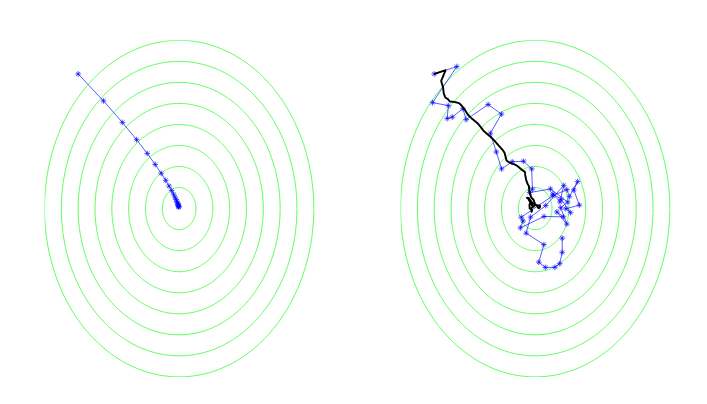
\includegraphics{figure_man/SGD.png}}
		\begin{tiny}\\ 
		Source: Shalev-Shwartz, Ben-David. Understanding machine learning. Cambridge University Press, 2014. 
		\end{tiny}\\
        Minimize $g(x_1, x_2) = 1.25(x_1 + 6)^2 + (x_2 - 8)^2)$. \\ Left: GD. Right: SGD, the black line depicts the averaged value of $\xv$.
	\end{figure}

	\framebreak 

        Assume batch size $m = 1$ (statements also apply for higher batch size).

	\begin{itemize}

		\item \textbf{(Possibly) suboptimal direction: }Approx. gradient $\bm{\hat d} = \nabla_\xv g_i(\xv)$ might point in suboptimal (possibly not even descent!) direction
		\item \textbf{Unbiased estimate: } If $J$ drawn i.i.d., approx. gradient $\bm{\hat d}$ is an unbiased estimate of gradient $\bm{d} = \nabla_\xv g(\xv) = \sumin \nabla_\xv g_i(\xv)$: 

		\vspace*{-0.5cm}

		\begin{eqnarray*}
			\mathbb{E}_{i}\left[\nabla_\xv ~g_i(\xv)\right] &=&\sumin \nabla_\xv ~g_i(\xv) \cdot \P(i = i) = \sumin \nabla_\xv ~ g_i(\xv) \cdot \frac{1}{n}\\ &=& \frac{1}{n} \sumin \nabla_\xv~g_i(\xv) = \nabla_\xv~ g(\xv).
		\end{eqnarray*}
	\end{itemize}
\textbf{Conclusion:} SGD might perform single suboptimal moves, but moves in \enquote{right direction} \textbf{on average}. 

\end{vbframe}

\begin{frame}{Erratic behavior of SGD}

\textbf{Example:}	$g(\xv) = \sum_{i = 1}^5 g_i(\xv)$, $g_i$ quadratic. We run SGD with $m = 1$. 

	\only<1>{
	\begin{figure}
			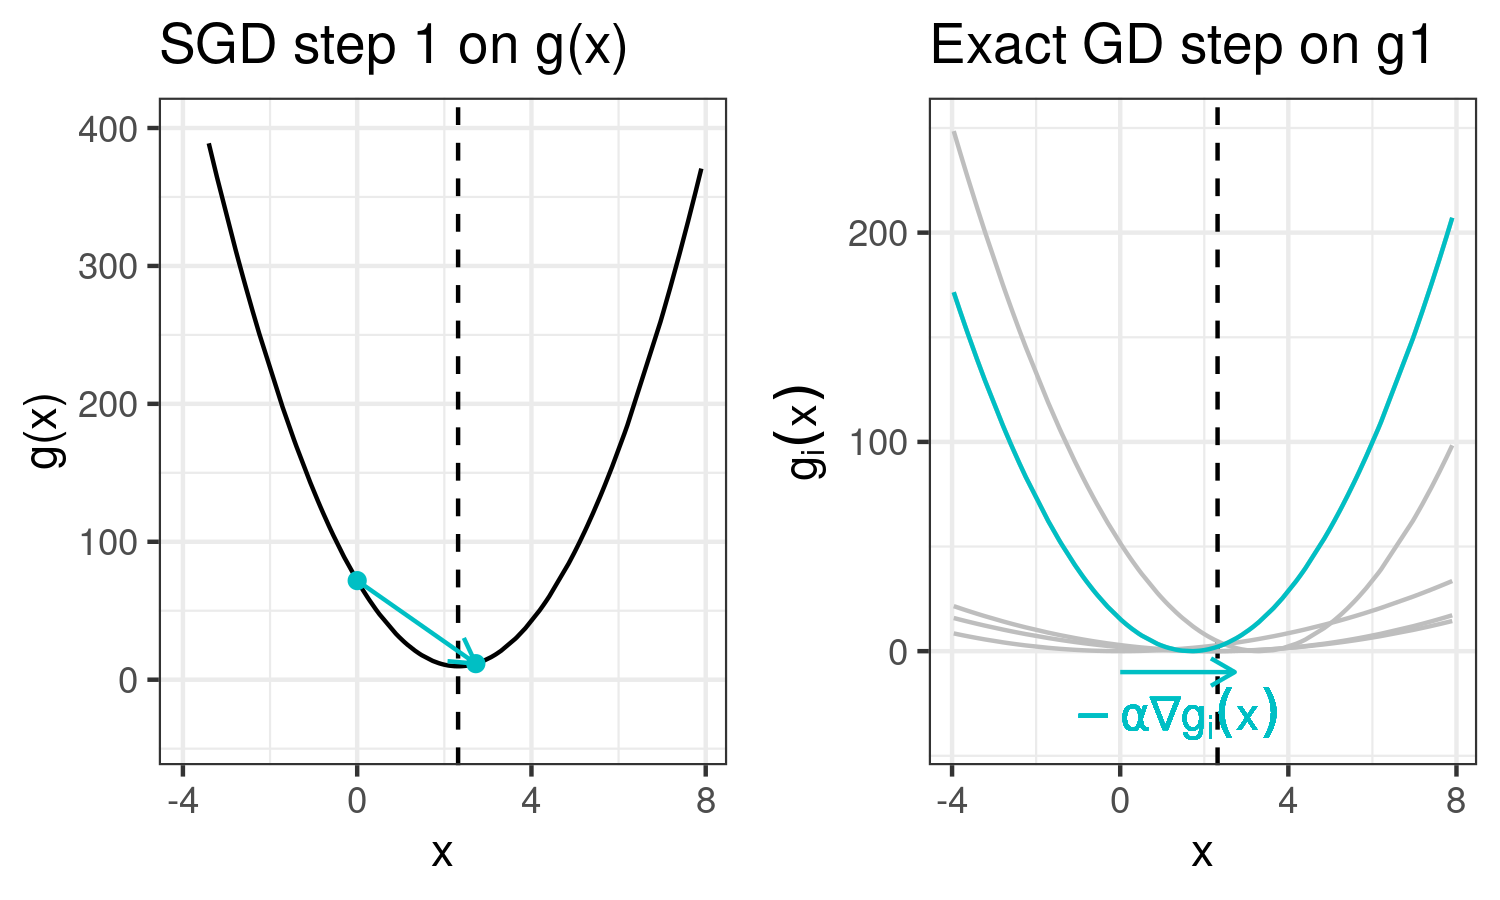
\includegraphics[width = 0.8\textwidth]{figure_man/sgd_example_iter_1.png}
	\end{figure}}
	\only<2>{
	\begin{figure}
			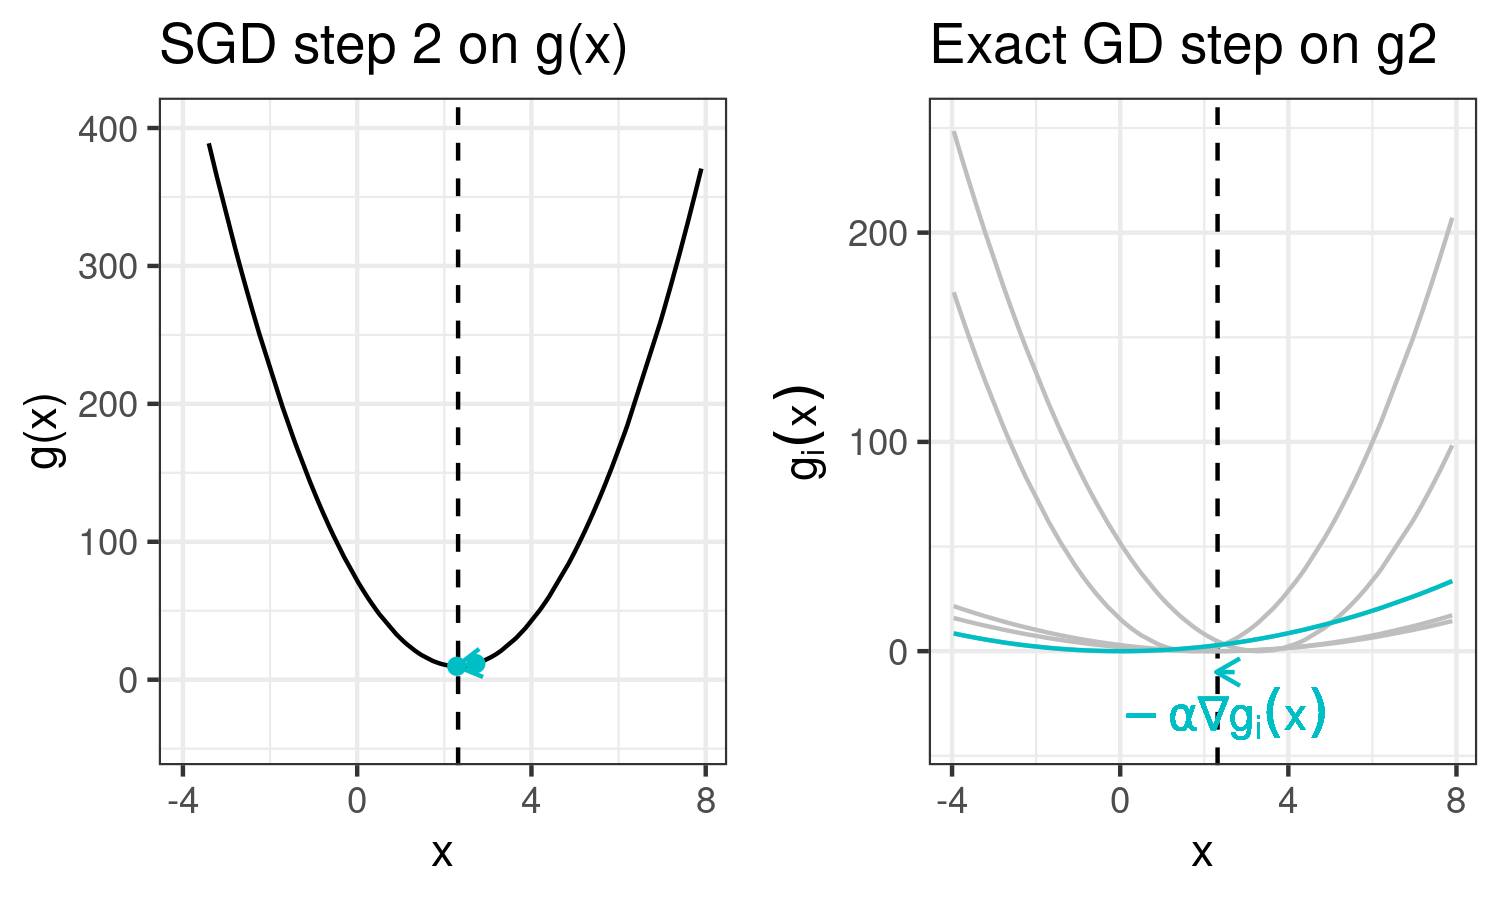
\includegraphics[width = 0.8\textwidth]{figure_man/sgd_example_iter_2.png}
	\end{figure}}
	\only<3>{
	\begin{figure}
			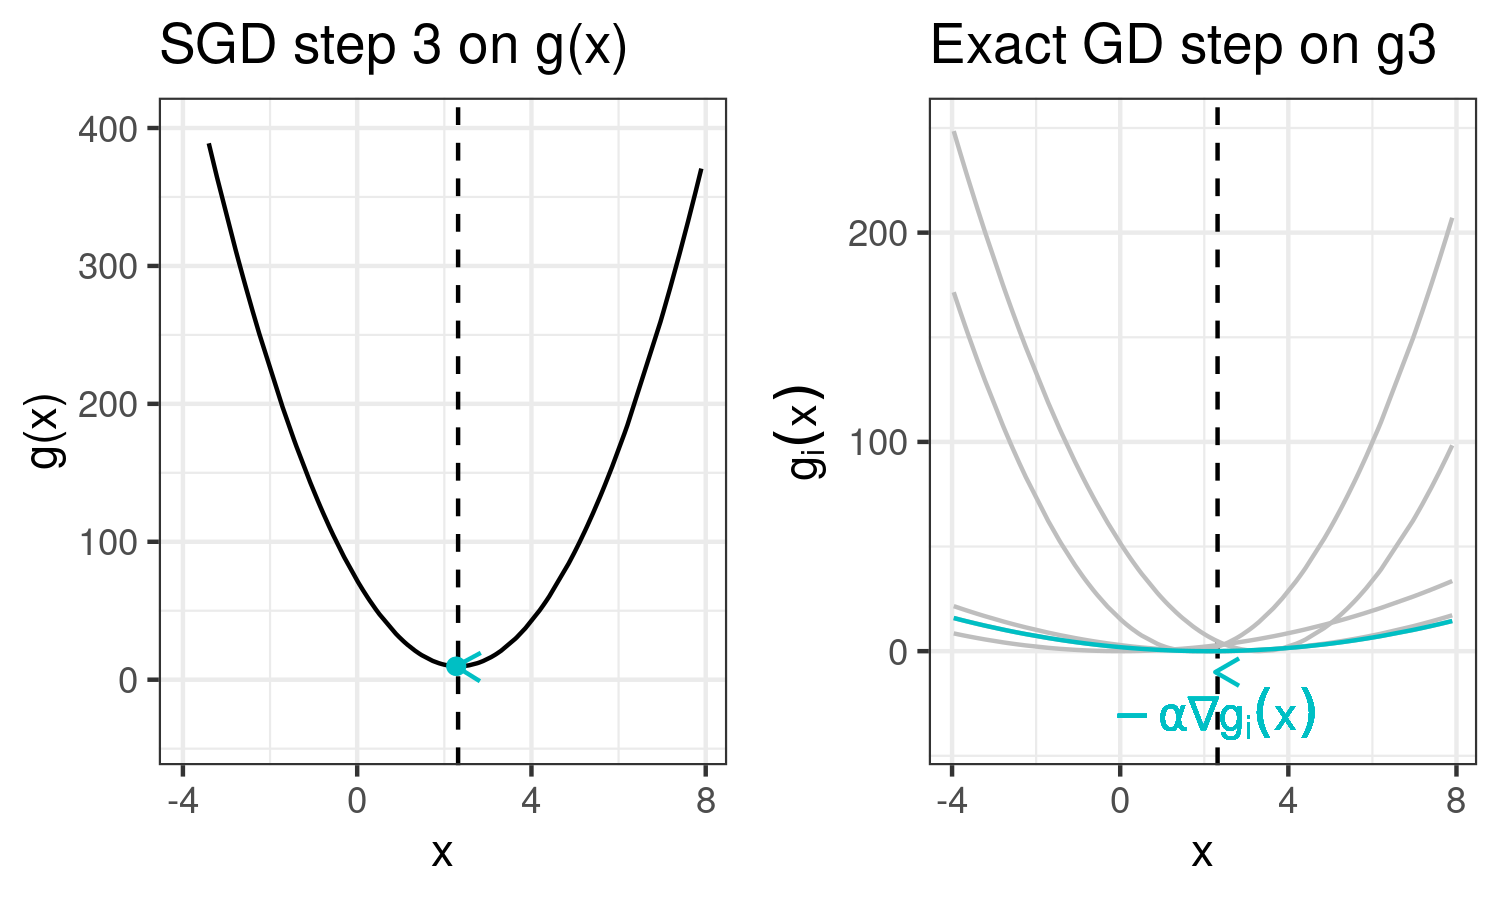
\includegraphics[width = 0.8\textwidth]{figure_man/sgd_example_iter_3.png}
	\end{figure}}
	\only<4>{
	\begin{figure}
			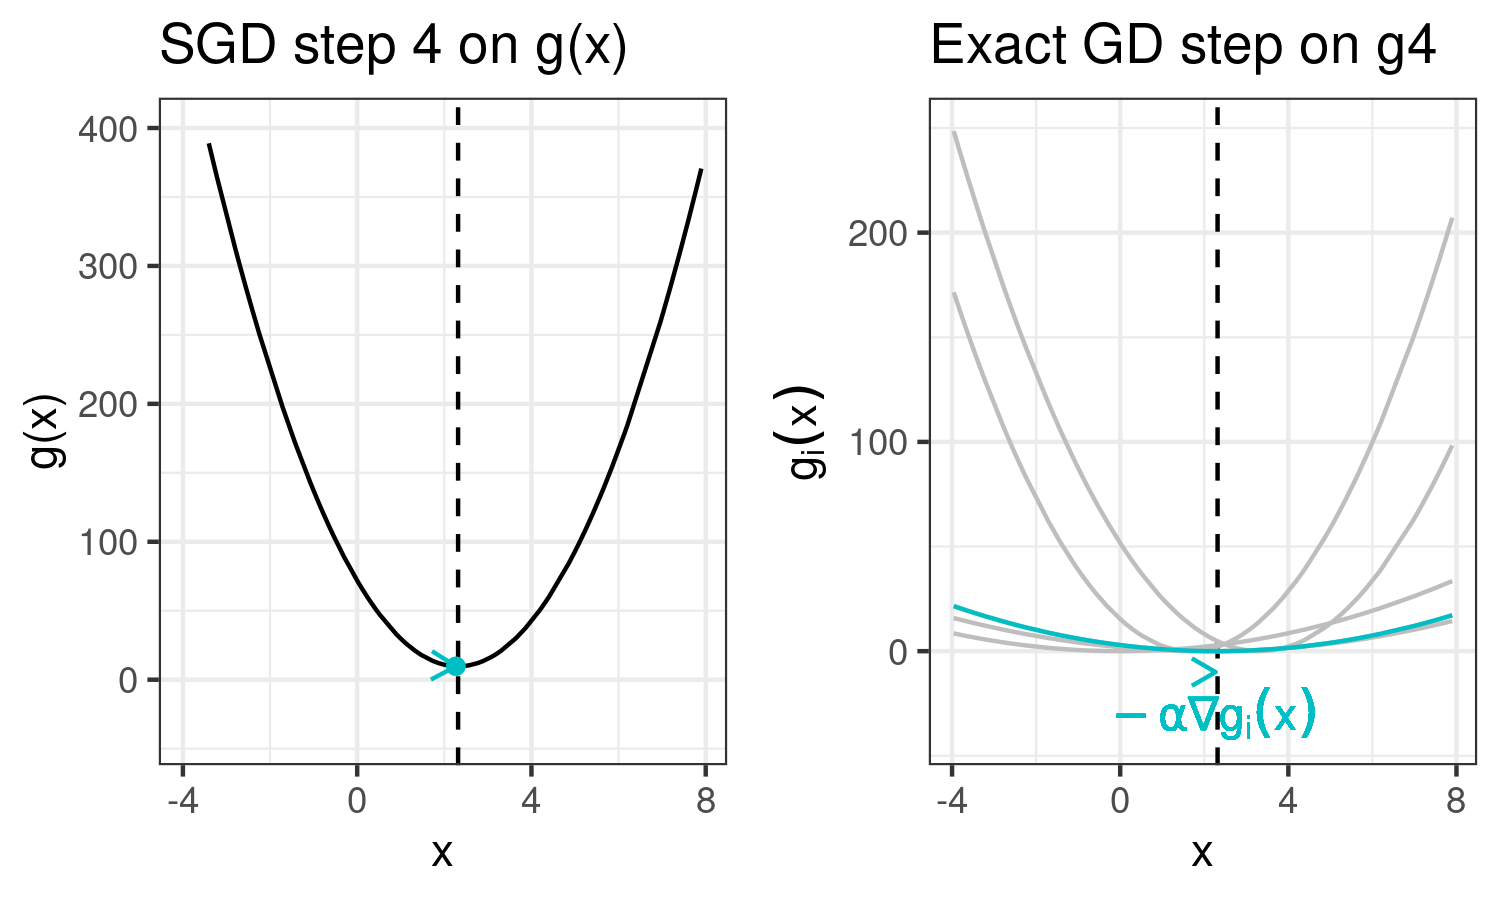
\includegraphics[width = 0.8\textwidth]{figure_man/sgd_example_iter_4.png}
	\end{figure}}
	\only<5>{
	\begin{figure}
			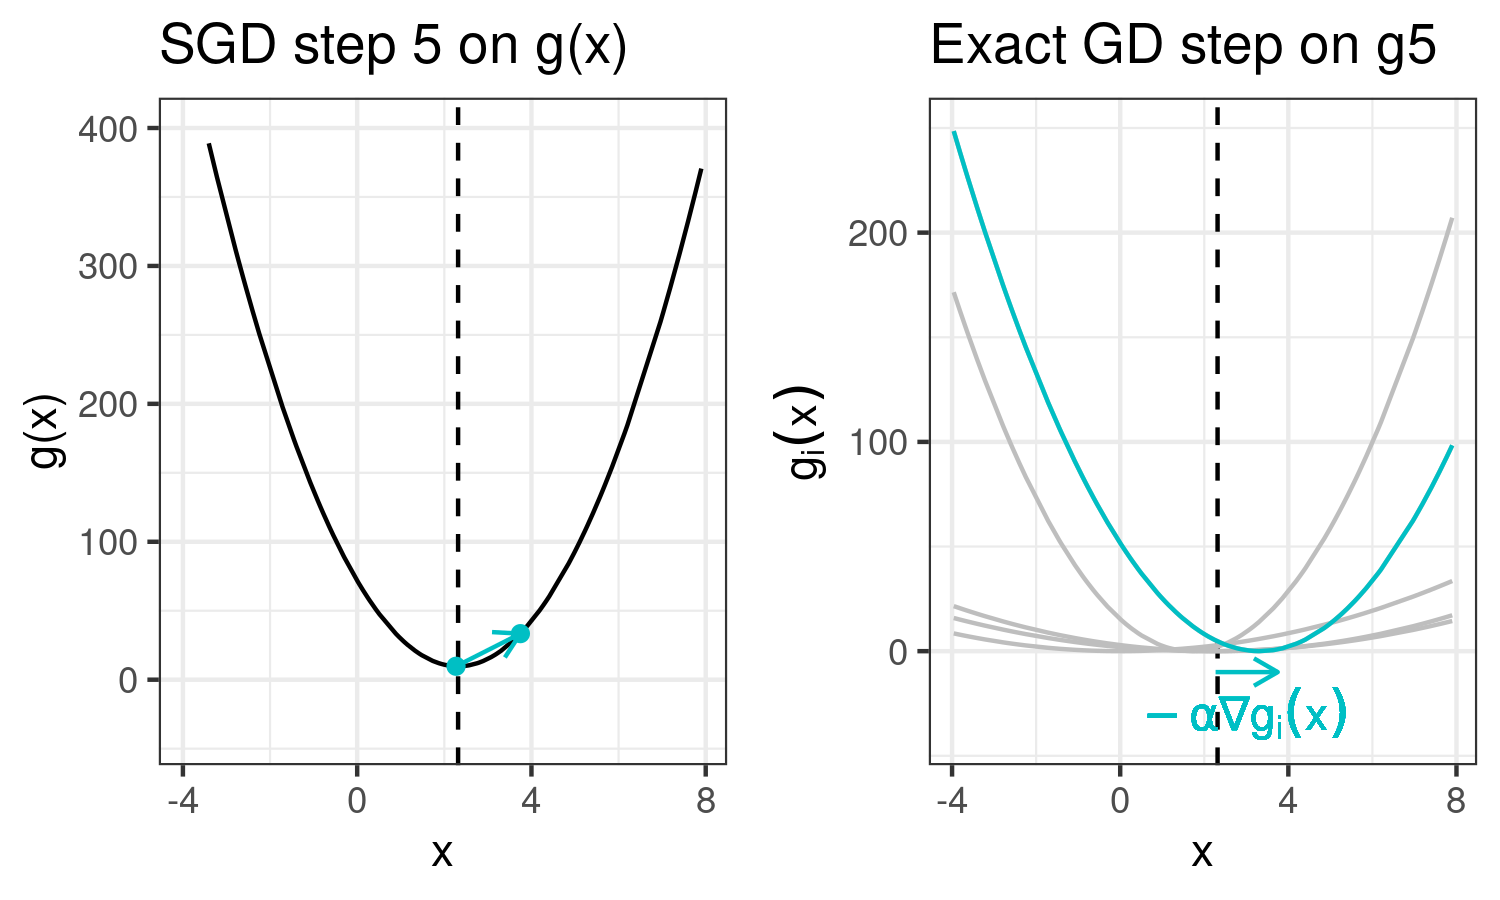
\includegraphics[width = 0.8\textwidth]{figure_man/sgd_example_iter_5.png} \\
			In iteration $5$, SGD performs a suboptimal move away from the optimum. 
	\end{figure}}
\end{frame}

\begin{vbframe}{Erratic behavior of SGD}

 	\begin{figure}
 		\vspace{-0.3cm}
 		\centering
 		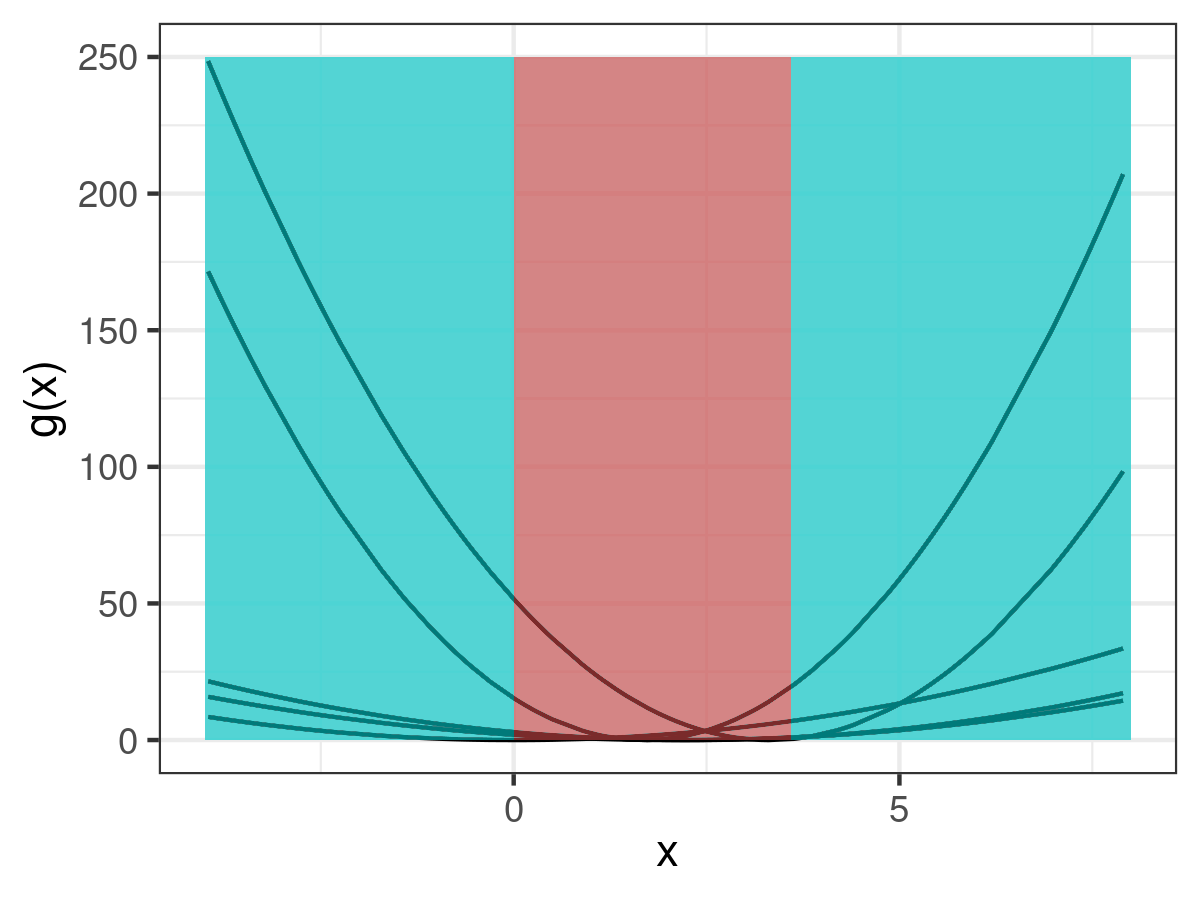
\includegraphics[width = 0.7\textwidth]{figure_man/sgd_example_confusion_areas.png} \newline
        \begin{footnotesize}
  $\xv$ in \textbf{blue area}: $- \nabla g_i(\xv)$ will point towards optimum, no matter which $i$ we sample. \\ $\xv$ in \textbf{red area} (confusion area): We might sample $i$ for which $- \nabla g_i(\xv)$ points away from optimum and perform suboptimal moves close to optimum. 
        \end{footnotesize}

  \end{figure}



 	\framebreak 

	\begin{itemize}
		\item At $\xv$, \enquote{confusion} is captured variance of gradients
		$$
			\frac{1}{n}\sumin \|\nabla_\xv~ g_i(\xv) - \nabla_\xv ~ g(\xv)\|^2
		$$
		\item If this variance is $0$, the next step will be in the right direction (independent of the sampled $i$)
		\item If the term is small, the next step will likely go in the right direction
		\item If the term is large, the step will likely go in the wrong direction (middle of confusion area, where $\xv^\ast$ lives)
	\end{itemize}

\end{vbframe}

\begin{vbframe}{Convergence of SGD}

	As a consequence, SGD has worse convergence properties than GD. However, this can be controlled via \textbf{increasing the batch size} or \textbf{reducing the step size}. 

	\begin{blocki}{The larger the batch size $m$}
		\item the better the approximation to $\nabla_\xv g(\xv)$
		\item the lower the variance
		\item the lower the risk of performing steps in the wrong direction
	\end{blocki}

	\begin{blocki}{The smaller the step size $\alpha$}
		\item the smaller a step in a potentially wrong direction 
		\item the lower the effect of high variance
	\end{blocki}


As maximum batch size is usually limited by computational resources (memory), choosing the step size is crucial. 

\end{vbframe}

\begin{vbframe}{Effect of batch size}

\begin{figure}
    \scalebox{0.9}{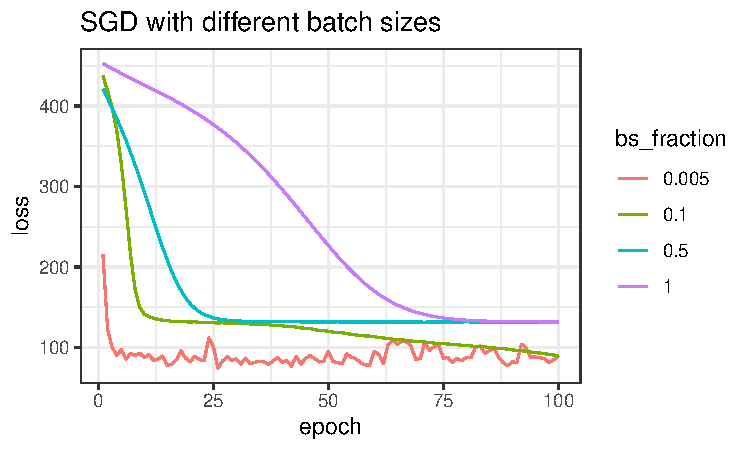
\includegraphics{slides/04-multivariate-first-order/figure_man/gradient_descent_NN_SGD_vs_no_SGD.pdf}} \\
    SGD to optimize an NN with batch size $\in \{0.5 \%, 10 \%, 50 \%\}$ \\ of the training data. 
    The higher the batch size, the lower the variance. 
\end{figure} 

\end{vbframe}


\endlecture
\end{document}

